% !TeX document-id = {4fba684d-7122-40d6-bb19-80adba5d32d5}
%!TeX TXS-program:compile = txs:///xelatex/
\documentclass{beamer}
\usetheme{Darmstadt}

\newif\ifproposal
\proposalfalse

\usepackage{standalone}

\usepackage{CJKutf8}

\usepackage[utf8]{inputenc}
\usepackage[OT1, T2A]{fontenc}
\usepackage{fontspec}
\setmainfont[ItalicFont={*},ItalicFeatures={FakeSlant=.167}]{D2Coding}

\usepackage[normalem]{ulem}

\usepackage{graphicx}
\usepackage{tikz}
\usetikzlibrary{quantikz}
\usepackage{braket}
\newcommand{\iu}{{i\mkern1mu}}

% based on the original definitions in beamerbasenavigation.sty
\makeatletter
\def\sectionentry#1#2#3#4#5{% section number, section title, page
    %
    \newcount\mymin%
    \mymin=3
    \ifnum\c@section=1%
    \mymin=5
    \fi%
    \ifnum\c@section=2%
    \mymin=4
    \fi%
    %
    \newcount\mymax%
    \mymax=3
    \ifnum\c@section=\beamer@sectionmax%
    \mymax=5
    \fi%
    \ifnum\c@section=\numexpr\beamer@sectionmax-1%
    \mymax=4
    \fi%
    %
    \ifnum\numexpr\c@section-#1<\mymax%
    \ifnum\numexpr#1-\c@section<\mymin%
    \ifnum#5=\c@part%
    \beamer@section@set@min@width
    \box\beamer@sectionbox\hskip1.875ex plus 1fill%
    \beamer@xpos=0\relax%
    \beamer@ypos=1\relax%
    \setbox\beamer@sectionbox=
    \hbox{
        \def\insertsectionhead{#2}%
        \def\insertsectionheadnumber{#1}%
        \def\insertpartheadnumber{#5}%

        {%
            \usebeamerfont{section in head/foot}\usebeamercolor[fg]{section in head/foot}%
            \ifnum\c@section=#1%
            \hyperlink{Navigation#3}{{\usebeamertemplate{section in head/foot}}}%
            \else%
            \hyperlink{Navigation#3}{{\usebeamertemplate{section in head/foot shaded}}}%
            \fi%
        }%
    }%
    \ht\beamer@sectionbox=1.875ex%
    \dp\beamer@sectionbox=0.75ex%
    \fi%
    \fi%
    \fi%
    \ignorespaces%
}

\def\slideentry#1#2#3#4#5#6{%
    %section number, subsection number, slide number, first/last frame, page number, part number
    %
    \newcount\mymin%
    \mymin=3
    \ifnum\c@section=1%
    \mymin=5
    \fi%
    \ifnum\c@section=2%
    \mymin=4
    \fi%
    %
    \newcount\mymax%
    \mymax=3
    \ifnum\c@section=\beamer@sectionmax%
    \mymax=5
    \fi%
    \ifnum\c@section=\numexpr\beamer@sectionmax-1%
    \mymax=4
    \fi%
    %
    \ifnum\numexpr\c@section-#1<\mymax%
    \ifnum\numexpr#1-\c@section<\mymin%
    \ifnum#6=\c@part\ifnum#2>0\ifnum#3>0%
    \ifbeamer@compress%
    \advance\beamer@xpos by1\relax%
    \else%
    \beamer@xpos=#3\relax%
    \beamer@ypos=#2\relax%
    \fi%
    \hbox to 0pt{%
        \beamer@tempdim=-\beamer@vboxoffset%
        \advance\beamer@tempdim by-\beamer@boxsize%
        \multiply\beamer@tempdim by\beamer@ypos%
        \advance\beamer@tempdim by -.05cm%
        \raise\beamer@tempdim\hbox{%
            \beamer@tempdim=\beamer@boxsize%
            \multiply\beamer@tempdim by\beamer@xpos%
            \advance\beamer@tempdim by -\beamer@boxsize%
            \advance\beamer@tempdim by 1pt%
            \kern\beamer@tempdim
            \global\beamer@section@min@dim\beamer@tempdim
            \hbox{\beamer@link(#4){%
                    \usebeamerfont{mini frame}%
                    \ifnum\c@section=#1%
                    \ifnum\c@subsection=#2%
                    \usebeamercolor[fg]{mini frame}%
                    \ifnum\c@subsectionslide=#3%
                    \usebeamertemplate{mini frame}%\beamer@minislidehilight%
                    \else%
                    \usebeamertemplate{mini frame in current subsection}%\beamer@minisliderowhilight%
                    \fi%
                    \else%
                    \usebeamercolor{mini frame}%
                    %\color{fg!50!bg}%
                    \usebeamertemplate{mini frame in other subsection}%\beamer@minislide%
                    \fi%
                    \else%
                    \usebeamercolor{mini frame}%
                    %\color{fg!50!bg}%
                    \usebeamertemplate{mini frame in other subsection}%\beamer@minislide%
                    \fi%
        }}}\hskip-10cm plus 1fil%
    }\fi\fi%
    \else%
    \fakeslideentry{#1}{#2}{#3}{#4}{#5}{#6}%
    \fi%
    \fi%
    \fi%
    \ignorespaces%
}
\makeatother

\AtBeginSection[]{
    \begin{frame}
        \vfill
        \centering
        \begin{beamercolorbox}[sep=8pt,center,shadow=true,rounded=true]{title}
            \usebeamerfont{title}\insertsectionhead\par%
        \end{beamercolorbox}
        \vfill
    \end{frame}
}

\usepackage{xcolor}
\usepackage{pgfplots}
\usepackage{tikz}

% Define bar chart colors
%
\definecolor{bblue}{HTML}{4F81BD}
\definecolor{rred}{HTML}{C0504D}
\definecolor{ggreen}{HTML}{9BBB59}
\definecolor{ppurple}{HTML}{9F4C7C}


\title{Quantum Speedup on Exhaustive-search Attacks on Cryptosystems}
%\subtitle{Week 7 Report for Class 75}

\author{2017320009 Sangheon Lee\\ 2017320023 Mingyu Cho}

\date{\today}

\begin{document}
    \begin{frame}
        \titlepage
    \end{frame}

    \begin{frame}
        \frametitle{Table of Contents}
        \tableofcontents
    \end{frame}

    \ifproposal
    \documentclass{beamer}
\usetheme{Darmstadt}
\usepackage{CJKutf8}

\usepackage[utf8]{inputenc}
\usepackage[OT1, T2A]{fontenc}
\usepackage{fontspec}
\usepackage[normalem]{ulem}

\usepackage{graphicx}
\usepackage{tikz}
\usepackage{braket}

\usepackage{xcolor}
\usepackage{pgfplots}
\usepackage{tikz}

\begin{document}
    \section{Necessity}

    \begin{frame}
        \frametitle{Necessity}

        \begin{itemize}
            \item ``Quantum Supremacy" imminent
            \item Post-quantum stage makes most cryptosystems used nowadays unsafe
            \begin{itemize}
                \item Prime factorization broken by Shor's Algorithm
            \end{itemize}
        \end{itemize}
    \end{frame}

    \section{Content}

    \begin{frame}
        \frametitle{Content}

        \begin{itemize}
            \item Targeting symmetric-key cryptosystem
            \begin{itemize}
                \item Specifically, DES will be used.
                \item If possible, make it able to be modified for any symmetric-key cryptosystems.
            \end{itemize}
            \item Brute-force exhaustive key search quantum algorithm
        \end{itemize}
    \end{frame}

    \section{Methods}

    \begin{frame}
        \frametitle{Methods}
        \begin{itemize}
            \item Modify Grover's Algorithm to crack DES
            \begin{itemize}
                \item $\Omega(\sqrt{n})$ search algorithm for a data table of $n$
            \end{itemize}
            \item Optionally, simulate it using projectq, a python-based quantum simulator
            \item Computationally determine and verify expected run-time, compare with existing attacks.
            \item Speed up if possible and/or necessary
        \end{itemize}
    \end{frame}

    \section{Expectations}

    \begin{frame}
        \frametitle{Expectations}

        \begin{itemize}
            \item The quantum algorithm will prove to be faster than at least the traditional brute-force exhaustive search.
            \item Planning to contrast two methods using the length of the key as a fixed variable if the algorithm is modifiable to others.
        \end{itemize}
    \end{frame}

    \section{Requirements}

    \begin{frame}
        \frametitle{Requirements}

        \begin{itemize}
            \item Papers and/or textbooks on quantum computation
            \item Help from Prof. Hong(He suggested the topic)
            \item[]
            \item Currently working with Sangheon Lee to study the backgrounds
            \item Agreed to study together before parting ways
        \end{itemize}
    \end{frame}

    \section{Backgrounds}

    \begin{frame}
        \frametitle{Mathematical Backgrounds}
        \begin{itemize}
            \item Complex numbers
            \begin{itemize}
                \item Complex plane $a+b\iu=(a,b)$
                \item Complex polar $\rho e^{\phi \iu}=\rho \cos \phi + \rho \sin \phi \iu$
            \end{itemize}
            \item 2-dimensional Hilbert space
            \begin{itemize}
                \item A complex vector space, utilizing conjugate transposes.
                \item When constricted to $\mathbb{R}$, same as $\mathbb{R}^2$ vector space.
            \end{itemize}
            \item Most of the time on Week 4 was spent on understanding the mathematical backgrounds on 2-dimensional Hilbert spaces and special matrices which can only be considered on $\mathbb{C}$.
            \item Additionally, analyzing Grover's Algorithm implementation in Microsoft Q\# was done.
        \end{itemize}
    \end{frame}

    \section{Qubits}
    \begin{frame}
        \frametitle{Qubits}
        \begin{itemize}
            \item Quantum Bit(Qubit for short) is a probabilistic vector of information.
            \item $\ket{0}=\begin{pmatrix} 1 \\ 0 \end{pmatrix}$, $\ket{1}=\begin{pmatrix} 0 \\ 1 \end{pmatrix}$
            \item A general qubit is represented as $u=\alpha \ket{0}+\beta \ket{1}$
        \end{itemize}
    \end{frame}

    \begin{frame}
        \frametitle{Three Main Types of Operation}
        \begin{itemize}
            \item Creation
            \item Reversible Operation
            \item Measurement
        \end{itemize}
    \end{frame}

    \begin{frame}
        \frametitle{Creation}
        \begin{itemize}
            \item As simple as creating $\ket{0}$ or $\ket{1}$.
        \end{itemize}
    \end{frame}

    \begin{frame}
        \frametitle{Reversible Operation}
        \begin{itemize}
            \item Represented using unitary matrix
            \begin{itemize}
                \item $U^*U=UU^*=I$, where $U^*$ is a conjugate transpose of $U$
            \end{itemize}
            \item Two frequently used operations
            \begin{itemize}
                \item X-gate $X=\begin{pmatrix} 0 & 1 \\ 1 & 0 \end{pmatrix}$ (so-called NOT gate)
                \item Hadamard Gate $H=\dfrac{1}{\sqrt{2}}\begin{pmatrix} 1 & 1 \\ 1 & -1 \end{pmatrix}$
                \item Hadamard Gate creates a Quantum Superposition
            \end{itemize}
        \end{itemize}
    \end{frame}

    \begin{frame}
        \frametitle{Measurement}
        \begin{itemize}
            \item A non-deterministic(probabilistic) measure of a qubit $u$.
            \item For a vector $u=\begin{pmatrix} \alpha \\ \beta \end{pmatrix}$ where $\|u\|=1$
            \begin{itemize}
                \item returns "true" with probability $\|\alpha\|^2$, and $u$ becomes $\ket{0}$
                \item returns "false" with probability $\|\beta\|^2$, and $u$ becomes $\ket{1}$
            \end{itemize}
            \item Destroys quantum superposition; often called "destructive".
        \end{itemize}
    \end{frame}
\end{document}
    \fi

    \section{S-DES}
    \documentclass{beamer}
\usetheme{Darmstadt}
\usepackage{CJKutf8}

\usepackage[utf8]{inputenc}
\usepackage[OT1, T2A]{fontenc}
\usepackage{fontspec}
\usepackage[normalem]{ulem}

\usepackage{graphicx}
\usepackage{tikz}
\usepackage{braket}

\usepackage{xcolor}
\usepackage{pgfplots}
\usepackage{tikz}

\begin{document}
    \begin{frame}{S-DES}
        \begin{itemize}
            \item Simplified DES with 2 rounds
            \item Structure similar to DES but simplified with 10-bit key and 8-bit plaintext.
            \item Quantum oracle needs to be reversible, of which S-DES is (normally) not.
        \end{itemize}
    \end{frame}

    \begin{frame}{Structure of S-DES}
        \begin{figure}[h]
            \centering
            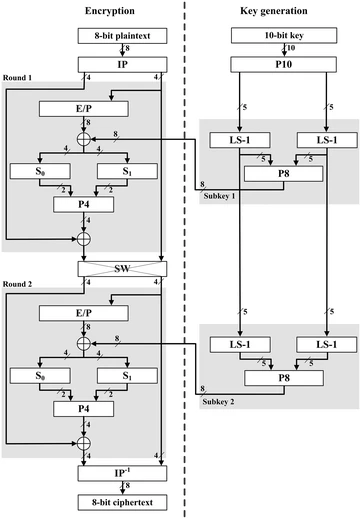
\includegraphics[width=0.5\textwidth]{./Images/sdes.png}
        \end{figure}
    \end{frame}

    \begin{frame}{Structure of S-DES}
        Consists of two main parts:
        \begin{itemize}
            \item Key Scheduling, where we generate subkeys from the given key
            \item Feistel function, where we encrypt the plaintext using the scheduled keys
        \end{itemize}
    \end{frame}

    \begin{frame}{Structure of S-DES: Key Scheduling}
        \begin{figure}[h]
            \centering
            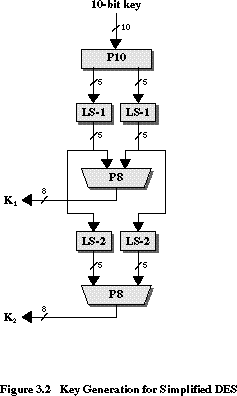
\includegraphics[width=0.5\textwidth]{./Images/keygen.png}
        \end{figure}
    \end{frame}

    \begin{frame}{Structure of S-DES: Feistel function}
        \begin{figure}[h]
            \centering
            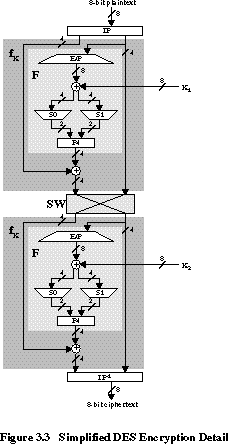
\includegraphics[width=0.38\textwidth]{./Images/feistel.png}
        \end{figure}
    \end{frame}

    \section{Grover's Algorithm}

    \begin{frame}{Overview}
        \begin{itemize}
            \item Grover's algorithm can find a specific state satisfying some condition among $ N = 2^n$ candidates in $ O(\sqrt{N}) $ time, compared to classical runtime complexity $ O(N) $.
            \item Grover's algorithm exploits qualities of quantum amplitudes to gain advantage of probability seperation.
            \item It can brute-force 128-bit symmetric cryptographic key in roughly $ 2^{64} $ iterations.
        \end{itemize}
    \end{frame}

    \begin{frame}{Algorithm}
        Input:
        \begin{itemize}
            \item A quantum oracle $ \mathcal{O} $ which performs the operation $ \mathcal{O} \ket{x}  = (-1)^{f(x)} \ket{x}$, where $ f(x) = 0 $ for all $0 \leq x < 2^n $ except $ x_0 $, for which $ f(x_0) = 1 $.
            \begin{itemize}
                \item Such quantum oracle is viable, and takes $ O(1) $ time.
            \end{itemize}
            \item $ n $ qubits initialized to the state $ \ket{0} $
        \end{itemize}
        Output: $ x_0 $, in runtime $ O(\sqrt{2^n}) $ with error rate $ O(\frac{1}{2^n}) $
    \end{frame}

    \begin{frame}{Algorithm}
        Procedure:
        \begin{enumerate}
            \item $ \ket{0}^{\otimes n} $ (initial state)
            \item $ H^{\otimes n} \ket{0}^{\otimes n} = \dfrac{1}{\sqrt{2^n}} \sum\limits_{x=0}^{2^n-1}\ket{x} = \ket{\psi}$ (Hadamard transform)
            \item $ [(2 \ket{\psi} \bra{\psi} - I) \mathcal{O}]^R \ket{\psi} \approx \ket{x_0}  $ (Grover iteration for $ R \approx  \frac{\pi}{4}\sqrt{2^n} $ times)
            \item $ x_0 $ (measure)
        \end{enumerate}
        Grover iteration in a nutshell: negate the amplitude of the desired state, followed by `diffusion transform' which increases the amplitude of the desired state and lower the others.
    \end{frame}
\end{document}

    \section{Quantum S-DES Oracle}
    \documentclass{beamer}
\usetheme{Darmstadt}
\usepackage{CJKutf8}

\usepackage[utf8]{inputenc}
\usepackage[OT1, T2A]{fontenc}
\usepackage{fontspec}
\usepackage[normalem]{ulem}

\usepackage{graphicx}
\usepackage{tikz}
\usetikzlibrary{quantikz}
\usepackage{braket}

\usepackage{xcolor}
\usepackage{pgfplots}
\usepackage{tikz}

\begin{document}
    \begin{frame}{Quantumizing S-DES}
        \begin{itemize}
            \item Most parts are permutations(or direct compressions); no problems here.
            \item Two parts pose a challenge:
	        \begin{enumerate}
	            \item Expansion
	            \item S-Boxes
	        \end{enumerate}
        \end{itemize}
    \end{frame}

    \begin{frame}{Dealing with Expansions}
        \begin{itemize}
            \item Due to \href{https://en.wikipedia.org/wiki/No-cloning_theorem}{No-cloning theorem}, directly copying a qubit is not possible.
            \item Use CNOT gate to perform XOR operation to copy the information.
        \end{itemize}
    \end{frame}

    \begin{frame}{Dealing with S-boxes}
        Consists of Lookup tables: Not ideal for quantum computing
        \begin{figure}[h]
            \centering
            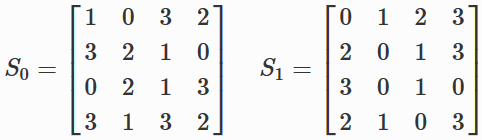
\includegraphics[width=0.5\textwidth]{./Images/sbox.png}
        \end{figure}
    \end{frame}

    \begin{frame}{Dealing with S-boxes: Quine-McCluskey Method}
        \begin{itemize}
            \item Break the S-Boxes into fundamental and/or/not-gates
            \item Letting the input bits into S-Boxes $ABCD$:
            \begin{itemize}
                \item S1 bit 1: $AB'C'+A'B'C+BCD'+ABD+BC'D$
                \item S1 bit 2: $AD'+B'D'+A'BC+ABC'$
                \item S2 bit 1: $AB'C'+ACD+A'CD'+A'BD'$
                \item S2 bit 2: $B'C'D+AB'C+BCD+BC'D'$
            \end{itemize}
            \item Directly calculating this would cause too many ancilla bits to use, i.e. for each and/or operation, one ancilla bit is required.
        \end{itemize}
    \end{frame}


    \begin{frame}{Dealing with S-boxes: The Brute-force Method}
    For each possibility in the S-box input, use a circuit similar to this:
    \begin{center}
    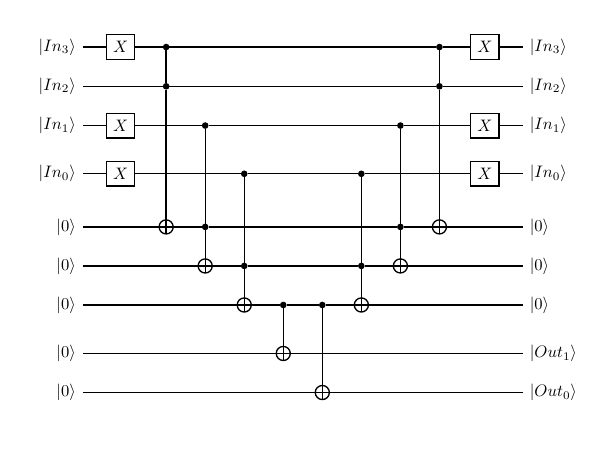
\begin{tikzpicture}
    \node[scale=0.6] {
    \begin{quantikz}
    \lstick{$\ket{In_3}$} & \gate{X} & \ctrl{1} & \qw & \qw & \qw & \qw & \qw & \qw & \ctrl{1} & \gate{X} & \qw  \rstick{$\ket{In_3}$} \\
    \lstick{$\ket{In_2}$} & \qw & \ctrl{3} & \qw & \qw & \qw & \qw & \qw & \qw & \ctrl{3} & \qw & \qw \rstick{$\ket{In_2}$} \\
    \lstick{$\ket{In_1}$} & \gate{X} & \qw & \ctrl{3} & \qw & \qw & \qw & \qw & \ctrl{3} & \qw & \gate{X} & \qw \rstick{$\ket{In_1}$} \\
    \lstick{$\ket{In_0}$} & \gate{X} & \qw & \qw & \ctrl{3} & \qw & \qw & \ctrl{3} & \qw & \qw & \gate{X} & \qw \rstick{$\ket{In_0}$} \\[0.2cm]
    \lstick{$\ket{0}$} & \qw & \targ{} & \ctrl{1} & \qw & \qw & \qw & \qw & \ctrl{1} & \targ{} & \qw & \qw \rstick{$\ket{0}$} \\
    \lstick{$\ket{0}$} & \qw & \qw & \targ{} & \ctrl{1} & \qw & \qw & \ctrl{1} & \targ{} & \qw & \qw & \qw \rstick{$\ket{0}$} \\
    \lstick{$\ket{0}$} & \qw & \qw & \qw & \targ{} & \ctrl{1} & \ctrl{2} & \targ{} & \qw & \qw & \qw & \qw \rstick{$\ket{0}$} \\[0.2cm]
    \lstick{$\ket{0}$} & \qw & \qw & \qw & \qw & \targ{} & \qw & \qw & \qw & \qw & \qw & \qw \rstick{$\ket{Out_1}$} \\
    \lstick{$\ket{0}$} & \qw & \qw & \qw & \qw & \qw & \targ{} & \qw & \qw & \qw & \qw & \qw \rstick{$\ket{Out_0}$}\\
    \end{quantikz}
    };
    \end{tikzpicture}
    \end{center}
    ...which requires 3 ancilla qubits.
    \end{frame}

    \begin{frame}{Dealing with S-boxes: The Brute-force Method}
    Thanks to the Microsoft Q\# library, we don't need that much ancilla qubits.
    \begin{center}
    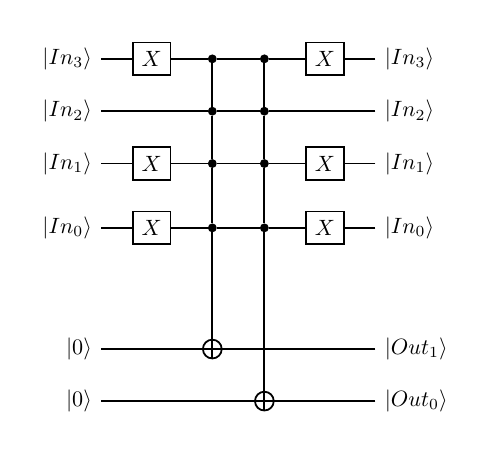
\begin{tikzpicture}
    \node[scale=0.8] {
    \begin{quantikz}
    \lstick{$\ket{In_3}$} & \gate{X} & \ctrl{1} & \ctrl{1} & \gate{X} & \qw \rstick{$\ket{In_3}$} \\
    \lstick{$\ket{In_2}$} & \qw & \ctrl{1} & \ctrl{1} & \qw & \qw \rstick{$\ket{In_2}$} \\
    \lstick{$\ket{In_1}$} & \gate{X} & \ctrl{1} & \ctrl{1} & \gate{X} & \qw \rstick{$\ket{In_1}$} \\
    \lstick{$\ket{In_0}$} & \gate{X} & \ctrl{1} & \ctrl{2} & \gate{X} & \qw \rstick{$\ket{In_0}$} \\[1cm]
    \lstick{$\ket{0}$} & \qw & \targ & \qw & \qw & \qw & \qw \rstick{$\ket{Out_1}$} \\
    \lstick{$\ket{0}$} & \qw & \qw & \targ & \qw & \qw & \qw  \rstick{$\ket{Out_0}$}
    \end{quantikz}
    };
    \end{tikzpicture}
    \end{center}
    No (explicit) ancilla qubits are required!
    \end{frame}

    \begin{frame}{Dealing with S-boxes: Combining the two methods?}
        \begin{itemize}
            \item Still a hypothetical yet.
            \item The structure of Quine-McCluskey simplified S-Box is similar to Brute-force
            \item The number of terms may decrease significantly, and one ancilla bit may be removed compared to the first circuit.
            \item Needs further testing...
        \end{itemize}
    \end{frame}
\end{document}

    \section{Quantum S-DES Implementation}
    \documentclass{beamer}
\usetheme{Darmstadt}
\usepackage{CJKutf8}

\usepackage[utf8]{inputenc}
\usepackage[OT1, T2A]{fontenc}
\usepackage{fontspec}
\usepackage[normalem]{ulem}

\usepackage{graphicx}
\usepackage{tikz}
\usetikzlibrary{quantikz}
\usepackage{braket}

\usepackage{xcolor}
\usepackage{pgfplots}
\usepackage{tikz}

\begin{document}
    \begin{frame}{Quantum S-DES Implementation}
        Initially, 34 explicit qubits were used in total.
        \begin{itemize}
            \item 10 qubits for input key
            \item 1 qubit for making an encryption oracle
            \item 8 qubits for (intermediate) plaintext
            \item 8 qubits for expanded plaintext
            \item 4 qubits for storing S-Box result
            \item 3 qubit for S-Box ancilla
        \end{itemize}
        S-DES implementation is written in Microsoft Q\#. Will it run?
    \end{frame}

    \begin{frame}{Quantum S-DES Implementation}
        Yes, and no.
        \begin{figure}[h]
            \centering
            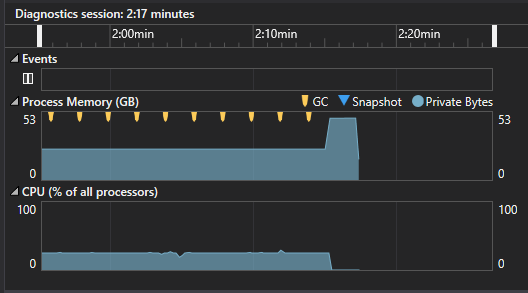
\includegraphics[height=0.5\textheight]{./Images/Qsharp-SDES-memory-error-2.png}
        \end{figure}
        After allocating 48GB of RAM, \texttt{System.Runtime.InteropServices.SEHException} was raised, indicating an out-of-memory error.
    \end{frame}

    \begin{frame}{Quantum S-DES Implementation}
        Reducing the number of qubits was necessary...!
        \begin{itemize}
            \item 10 qubits for input key
            \item 1 qubit for making an encryption oracle
            \item 8 qubits for (intermediate) plaintext
            \item \only<1>{8 qubits for expanded plaintext} \only<2->{{\color{gray}\sout{8 qubits for expanded plaintext}}}
            \item \only<1-2>{4}\only<3->{{\color{gray}\sout{4}} 2} qubits for storing S-Box result
            \item \only<-3>{3 qubits for S-Box ancilla} \only<4>{{\color{gray}\sout{3 qubits for S-Box ancilla}}}
        \end{itemize}
        \onslide<2-> We can directly use plaintext qubits to create result qubits from S-Box. After then we can undo all the operations (permutation, \textit{etc.}) which altered plaintext.

        \onslide<3->Additionally, each S-Box operation is independent. Thus we can reuse S-box result qubits after re-initialization.

        \onslide<4->Finally, redundant S-Box ancilla qubits were removed.
    \end{frame}


    \begin{frame}{Quantum S-DES Implementation}
        However, applying Grover's was not simple as it looked
        \begin{itemize}
            \item The oracle should be adjoint, but original version includes measurement (in result ciphertext and S-Box)
            \item How to create an oracle qubit rather than measuring the result ciphertext?
            \begin{itemize}
                \item perform CNOT gate 8 times (with 7 more qubits) : infeasible
                \item Microsoft Q\#'s \texttt{Controlled} functor : doable
            \end{itemize}
            \item Similar to S-Box Controlling
            \item S-Box also required measurement initially, but change to forementioned circuit
        \end{itemize}
        Result : reversible S-DES oracle.

    \end{frame}

    \begin{frame}{Quantum S-DES Implementation}
        \begin{figure}
            \centering
            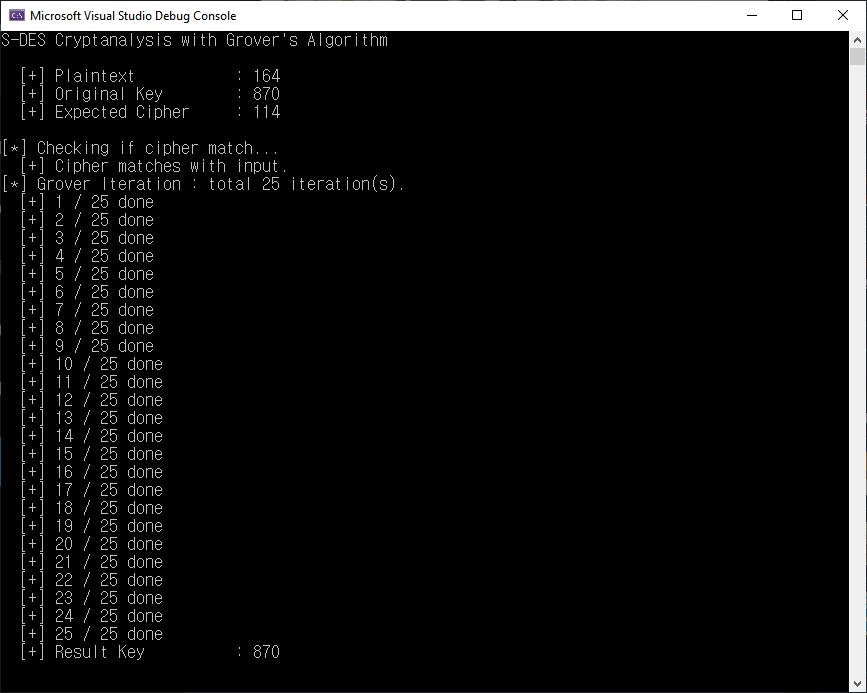
\includegraphics[height=0.5\textheight]{./Images/Qsharp-SDES-Grover-k1.png}
        \end{figure}
        Expected key matched with original key (with runtime 1 min 12 sec, performing each S-DES encryption within 2-3s on average).
    \end{frame}
\end{document}

    \section{Quantum S-DES Testing}
    \documentclass{beamer}
\usetheme{Darmstadt}
\usepackage{CJKutf8}

\usepackage[utf8]{inputenc}
\usepackage[OT1, T2A]{fontenc}
\usepackage{fontspec}
\usepackage[normalem]{ulem}

\usepackage{graphicx}
\usepackage{tikz}
\usetikzlibrary{quantikz}
\usepackage{braket}

\usepackage{xcolor}
\usepackage{pgfplots}
\usepackage{tikz}

\begin{document}
    \begin{frame}{Prerequisites}
        \begin{itemize}
            \item Let $ SDES(P, K) = C $ be a function s.t. encrypting plaintext $ P $ with S-DES and key $ K $ yields $ C $.
            \item Let $ f : \{0, 1\}^8 \times \{0, 1\}^8 \to \mathcal{P}({\{0, 1\}^{10}})$ be a function such that $ f(P, C) = \{ K \in \{0, 1\}^{10} \,\vert\, SDES(P, K) = C\}$.
            \item Since key size is 4x of cipher size, we guessed that for arbitrary $ P $ and $ C $, $ \left\vert f(P, C) \right\vert$ is likely to be 4.
        \end{itemize}
    \end{frame}

    \begin{frame}{Prerequisites : Key Size}
        ...and we were wrong!
        % include graph here
        \begin{tikzpicture}
            \begin{axis}[
                width  = 0.95*\textwidth,
                height = 0.8\textheight,
%                major x tick style = transparent,
                ybar,
                bar width=6pt,
                ymajorgrids = true,
                ylabel = {\# of $ (P, C) $ pairs},
                xlabel = {Key size},
                symbolic x coords={1,2,3,4,5,6,7,8,9,10,11,12,13,14,15,16,17},
                xtick = data,
                enlarge x limits=0.05,
                ymin=0,
                ymode=log,
            ]

                \addplot[style={bblue,fill=bblue,mark=none}]
                    coordinates {
                        (1, 4376)
                        (2, 10696)
                        (3, 6888)
                        (4, 11896)
                        (5, 3848)
                        (6, 9576)
                        (7, 2728)
                        (8, 4184)
                        (9, 968)
                        (10, 1944)
                        (11, 272)
                        (12, 456)
                        (13, 16)
                        (14, 24)
                        (15, 96)
                        (16, 8)
                        (17, 8)
                        };
            \end{axis}
        \end{tikzpicture}
    \end{frame}

    \begin{frame}{Quantum S-DES Testing : Testing with \#Key = 1}
        If $ (P, C) =$ (\texttt{10100100}, \texttt{00110011}). Then $ f(P, C) = $  $\{$\texttt{1101100110}$\}$.
        \begin{itemize}
            \item Program yielded correct key.
            \item By dumping key qubits, we can observe the probability of each basis.
            \begin{itemize}
                \item At first, the probability of answer basis is $ 0.008766 $ while the others are $ 0.000969 $.
                \item The gap widens next turn: $ 0.024224 $ and $ 0.000954 $.
                \item Ultimately it becomes $ 0.999461 $ and $ 0.000001 $ (at 25th iteration).
            \end{itemize}
        \end{itemize}
    \end{frame}


    \begin{frame}{Quantum S-DES Testing : Testing with \#Key = 4}
        If $ (P, C) =$ (\texttt{11000111}, \texttt{00010100}). Then $ \vert f(P, C) \vert = 4$.
        \begin{itemize}
            \item Program yielded wrong key.
            \item By dumping key qubits, we can observe the probability of each basis.
            \begin{itemize}
                \item At first, the probability of answer basis is $ 0.008698 $ while the others are $ 0.000946 $.
                \item The gap widens next turn: $ 0.023659 $ and $ 0.000888 $.
                \item It peaks at 12th iteration: $ 0.249987 $ and $ 0.000000 $.
                \item However it goes back next turn: $ 0.246547 $ and $ 0.000014 $
                \item Ultimately the probability of answer basis becomes lower than the others: $ 0.000575 $ and $ 0.000978 $.
            \end{itemize}
            \item Although the algorithm and the implementation is correct, what happened here? % 논문 추가
        \end{itemize}
    \end{frame}

    \begin{frame}{Quantum S-DES Testing: What Went Wrong?}
        \begin{itemize}
            \item When running Grover's Algorithm, there is a number of desired steps, say $n$.
            \item If we overshoot that number of step, the probability of basis decreases!
            \item On the $2n$-th step, the probability becomes all the same for each of the cases again, forming a cycle.
        \end{itemize}
    \end{frame}
\end{document}

    \section{Quantum S-DES Gate Analysis}
    \documentclass{beamer}
\usetheme{Darmstadt}
\usepackage{CJKutf8}

\usepackage[utf8]{inputenc}
\usepackage[OT1, T2A]{fontenc}
\usepackage{fontspec}
\usepackage[normalem]{ulem}

\usepackage{graphicx}
\usepackage{tikz}
\usetikzlibrary{quantikz}
\usepackage{braket}

\usepackage{xcolor}
\usepackage{pgfplots}
\usepackage{tikz}

\begin{document}
	\begin{frame}{Overview}
		\begin{itemize}
			\item Most part can be expressed in permutations, but there are parts where we need to use quantum gates.
			\item In S-Box, we inevitably need to use Pauli-X and Toffoli gates.
			\item In EP, we need to copy the bits, and thereby requires the use of Toffoli gates.
			\item In round application, we need to XOR the subkey with some data or S-box result, requiring us to use CNOT gates.
		\end{itemize}
	\end{frame}
	
	\begin{frame}{Number of Gates: Brute-forcing S-Box}
		\begin{itemize}
			\item Both S-box requires certain number of Pauli-X and Toffoli(CCNOT) gates.
			\item The sum of gates required for each of the 16 inputs possible:
			\begin{center}
				\begin{tabular}{c|c|c}
					        & Pauli-X & Toffoli \\\hline
					S-box 1 & 50      & 18      \\\hline
					S-box 2 & 44      & 15
				\end{tabular}
			\end{center}
			\item On average, \textasciitilde3 Pauli-X gates and \textasciitilde1 Toffoli gate is used.
		\end{itemize}
	\end{frame}
	
	\begin{frame}{Number of Gates: Quine-McCluskey S-Box}
		\begin{itemize}
			\item What about Quine-McCluskey Method?
			\item Looking at S-boxes:
			\begin{itemize}
				\item S1 bit 1: $AB'C'+A'B'C+BCD'+ABD+BC'D$
				\item S1 bit 2: $AD'+B'D'+A'BC+ABC'$
				\item S2 bit 1: $AB'C'+ACD+A'CD'+A'BD'$
				\item S2 bit 2: $B'C'D+AB'C+BCD+BC'D'$
			\end{itemize}
			\item Only OR operations need to be done with Toffoli gates; AND operations can be done the same way as Brute-force.
			\item For any given input, exactly the following number of operations are required in naïve approach:
			\begin{center}
				\begin{tabular}{c|c|c}
					& NOT & OR \\\hline
					S-box 1 & 11      & 7      \\\hline
					S-box 2 & 10      & 6
				\end{tabular}
			\end{center}
			\item TODO
		\end{itemize}
	\end{frame}
	
	\begin{frame}{Number of Gates: S-Box Input and Output}
		\begin{itemize}
			\item For input, 4 CNOT gates are required.
			\item To copy the output, 2 more CNOT gates are required.
			\item To make this reversible, S-box application and input processes must be reversed, requiring 2 S-Box applications and 8 CNOT gates.
			\item[$\Rightarrow$] Total of 10 CNOT gates, along with two S-box applications.
		\end{itemize}
	\end{frame}
	
	\begin{frame}{Number of Gates: Apply Rounds}
		\begin{itemize}
			\item Both S-boxes are applied per round, scoring in for 20 CNOT gates, 94 Pauli-X gates, and 33 Toffoli gates.
			\begin{itemize}
				\item The remaining operations are all permutations.
			\end{itemize}
			\item There are two rounds in total.
			\item[$\Rightarrow$] Total of 40 CNOT gates, 188 Pauli-X gates, and 66 Toffoli gates per single oracle call!
		\end{itemize}
	\end{frame}
\end{document}
\ifproposal
    \section{Current Works and Future Plans}
    \documentclass{beamer}
\usetheme{Darmstadt}
\usepackage{CJKutf8}

\usepackage[utf8]{inputenc}
\usepackage[OT1, T2A]{fontenc}
\usepackage{fontspec}
\usepackage[normalem]{ulem}

\usepackage{graphicx}
\usepackage{tikz}
\usetikzlibrary{quantikz}
\usepackage{braket}

\usepackage{xcolor}
\usepackage{pgfplots}
\usepackage{tikz}

\begin{document}
\begin{frame}
        \frametitle{Work in Progress(Mingyu Cho)}
        \begin{itemize}
            \item Implemented a non-quantum S-DES(in python) for testing the quantum version.
            \item Implemented Brute-force attack on S-DES and developed a code for keycount for (plaintext, ciphertext) pair.
            \item Started preliminary analysis on the gate applications
            \item Looking for possible speedups on the quantum side to aid the simulation
        \end{itemize}
    \end{frame}

    \begin{frame}
        \frametitle{Work in Progress(Sangheon Lee)}
        \begin{itemize}
            \item Possibly reduce some quantum gates
            \item Analyze complexity of each gate
            \item Search for internal dumping library
        \end{itemize}
    \end{frame}

    \begin{frame}
        \frametitle{Future Plans}
        \begin{itemize}
            %\item Dig in deeper on the backgrounds, if necessary.
            %\item Understand Grover's Algorithm and other quantum algorithms to know how to utilize it.
            %\item Update sample code of Grover's Algorithm by implementing oracle function and randomization.
            %\item Possibly utilize IBM Quantum Experience?
            %\item Search some more sample codes (not sure if implementing and debugging Shor's and QFT is necessary).
            \item Construct and test S-DES and apply Grover's.
            \begin{itemize}
                \item Since S-DES consists of various components, all of these must be implemented carefully and in order
            \end{itemize}
            \item Hope to import Microsoft Q\# implementation to qiskit (IBM Quantum Experience)
            \item Reduce complexity of quantum gates if possible (as Prof. Hong suggested)
        \end{itemize}
    \end{frame}
\end{document}
\fi
\end{document}